\section{Chi-squared Distribution}


\subsection{Standard Chi-squared distribution}

The pdf is

\begin{equation}
	f(x, k) = \frac{1}{2^{k/2}\Gamma(k/2)}  x^{k/2 -1} \exp(-x/2)
	\label{eq:chi2_pdf}
\end{equation} 

which can be written as

\begin{equation}
	f(x, k) = \exp \left[(k/2-1)\log(x) - x/2 - \log(2^{k/2}\Gamma(k/2))\right]
	\label{eq:chi2_exp_family}
\end{equation}

with $T = (\log(x), x), \eta = (k/2 - 1)$ and $A(k) = \log(2^{k/2}\Gamma(k/2))$.

\subsubsection{Laplace approximation of the standard Chi-squared distribution}

\begin{align*}
\text{log-pdf: } &(k/2-1)\log(x) - x/2 - \log(2^{k/2}\Gamma(k/2)) \\
\text{1st derivative: }&  \frac{k/2-1}{x} - \frac{1}{2} \\
\text{mode: }&  \frac{k/2-1}{x} - \frac{1}{2} = 0 \Leftrightarrow x = k-2\\
\text{2nd derivative: }&  -\frac{k/2-1}{x^2}\\
\text{insert mode: }& -\frac{k/2-1}{(k-2)^2}\\
\text{invert and times -1: }&\sigma^2 = \frac{(k-2)^2}{k/2 -1}
\end{align*}

\subsection{Log-Transformed Chi-squared distribution}

we transform the distribution with $g(x) = \log(x)$, i.e. $g^{-1}(x) = \exp(x)$. The new pdf becomes

\begin{equation}
	f_t(x,k) = \frac{1}{2^{k/2}\Gamma(k/2)}  \exp(x)^{k/2 -1} \exp(-\exp(x)/2)
	\label{eq:chi2_trans_pdf}
\end{equation}

which can be written as

\begin{equation}
	f_t(x, k) = \exp \left[(k/2)x - \frac{\exp(x)}{2} - \log(2^{k/2}\Gamma(k/2)) \right]
	\label{eq:chi2_trans_exp_family}
\end{equation}

meaning $T=(x, \exp(x)), \eta=(k/2)$ and $A(k) =  \log(2^{k/2}\Gamma(k/2))$. 

\subsubsection{Laplace approximation of the log-transformed Chi-squared distribution}

\begin{align*}
\text{log-pdf: } &(k/2)x - \frac{\exp(x)}{2} - \log(2^{k/2}\Gamma(k/2)) \\
\text{1st derivative: }&  k/2 - \frac{\exp(x)}{2} \\
\text{mode: }& k/2 - \frac{\exp(x)}{2} = 0 \Leftrightarrow x = \log(k)\\
\text{2nd derivative: }&  -\frac{\exp(x)}{2}\\
\text{insert mode: }& -k/2\\
\text{invert and times -1: }&\sigma^2 = 2/k
\end{align*}

\subsubsection{The Bridge for log-transform}

\begin{align}
	\mu &= \log(k) \\
	\sigma^2 &= 2/k \\
	k &= \exp(\mu)
\end{align}

\begin{figure}[!htb]
	\centering
	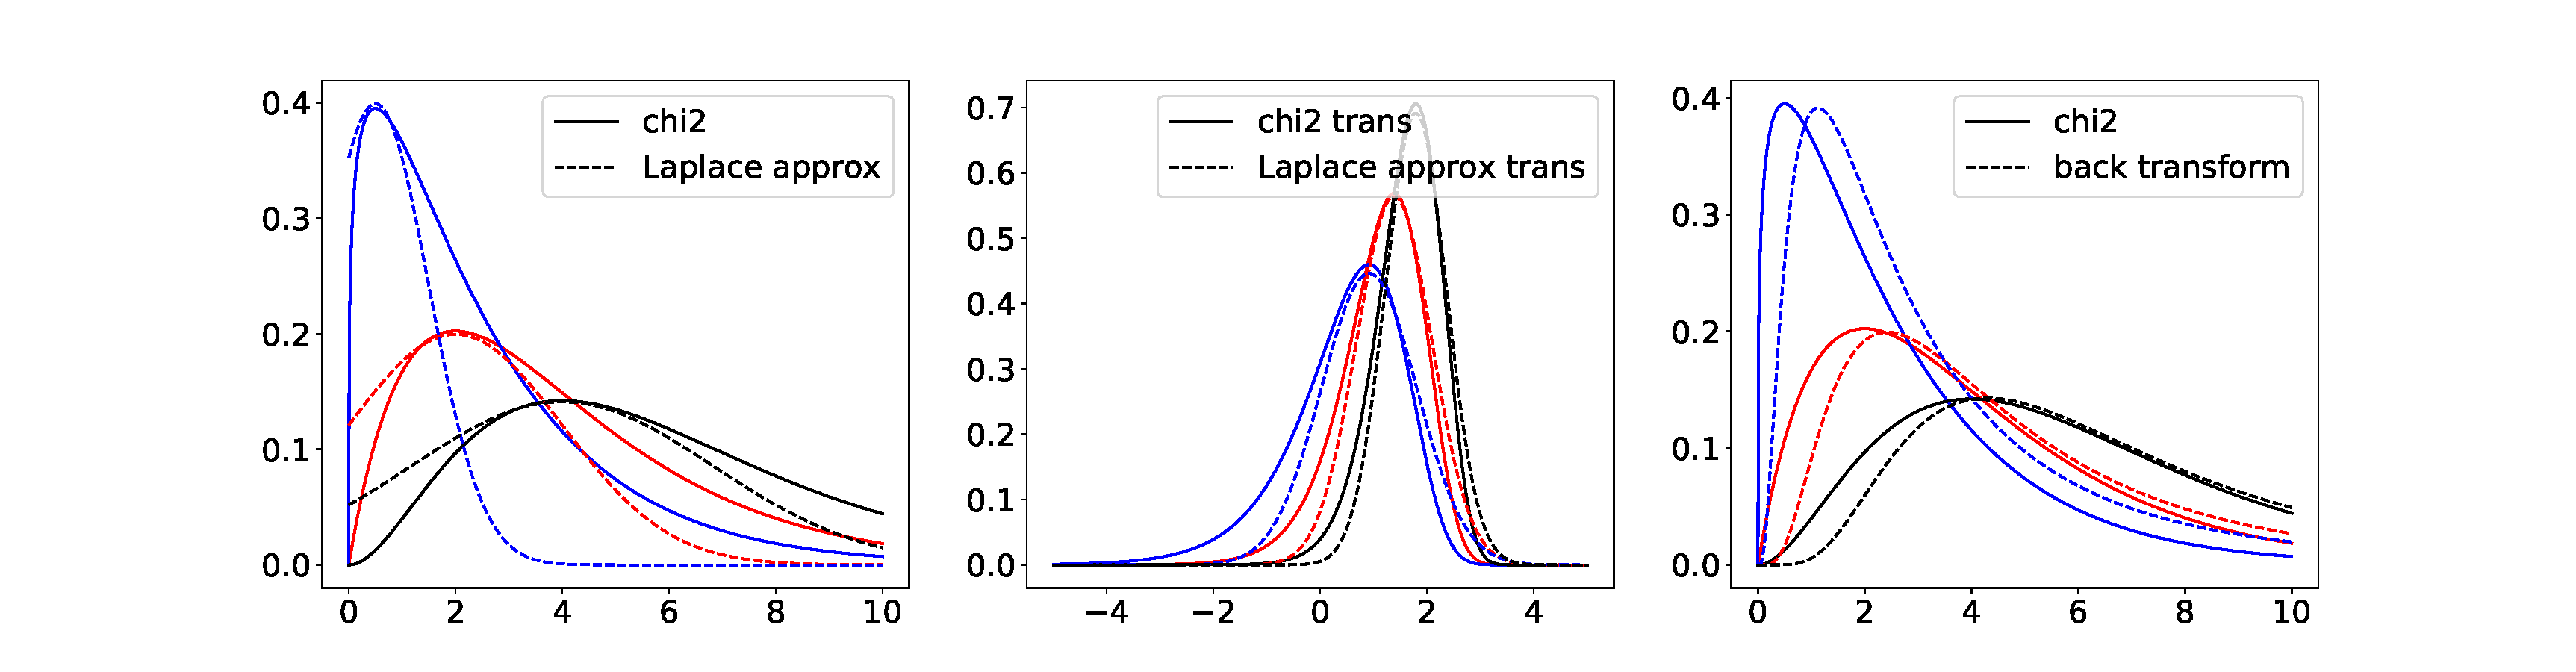
\includegraphics[width=\textwidth]{figures/chi2_playground_log.pdf}
	\caption{chi2 comparison log transform}
	\label{fig:chi2_log_comparison}
\end{figure}

\subsection{Sqrt-Transformed Chi-squared distribution}

we transform the distribution with $g(x) = \sqrt{x}$, i.e. $g^{-1}(x) = x^2$. The new pdf becomes

\begin{align}
f_t(x,k) &= \frac{1}{2^{k/2}\Gamma(k/2)}  x^{2(k/2 -1)} \exp(-x^2/2)  2x\\ \nonumber
		 &= \frac{1}{2^{k/2}\Gamma(k/2)}  x^{k} \exp(-x^2/2)
\label{eq:chi2_sqrt_trans_pdf}
\end{align}

which can be written as

\begin{equation}
f_t(x, k) = \exp \left[(k\log(x) - \frac{x^2}{2} - \log(2^{k/2}\Gamma(k/2)) \right]
\label{eq:chi2_sqrt_trans_exp_family}
\end{equation}

meaning $T=(\log(x), x^2), \eta=(k, 1/2)$ and $A(k) =  \log(2^{k/2}\Gamma(k/2))$. 

\subsubsection{Laplace approximation of the sqrt-transformed Chi-squared distribution}

\begin{align*}
\text{log-pdf: } &(k\log(x) - \frac{x^2}{2} - \log(2^{k/2}\Gamma(k/2)) \\
\text{1st derivative: }&  \frac{k}{x} -x \\
\text{mode: }& \frac{k}{x} -x = 0 \Leftrightarrow x = \sqrt{k}\\
\text{2nd derivative: }&  -\frac{k}{x^2} - 1\\
\text{insert mode: }& -\frac{k}{k}-1\\
\text{invert and times -1: }&\sigma^2 = 1/2
\end{align*}

\subsubsection{The Bridge for sqrt-transform}

\begin{align}
\mu &= \sqrt{k} \\
\sigma^2 &= 1/2 \\
k &= \mu^2
\end{align}

TODO:THE BRIDGE BACK LOOKS A BIT WEIRD\\

\begin{figure}[!htb]
	\centering
	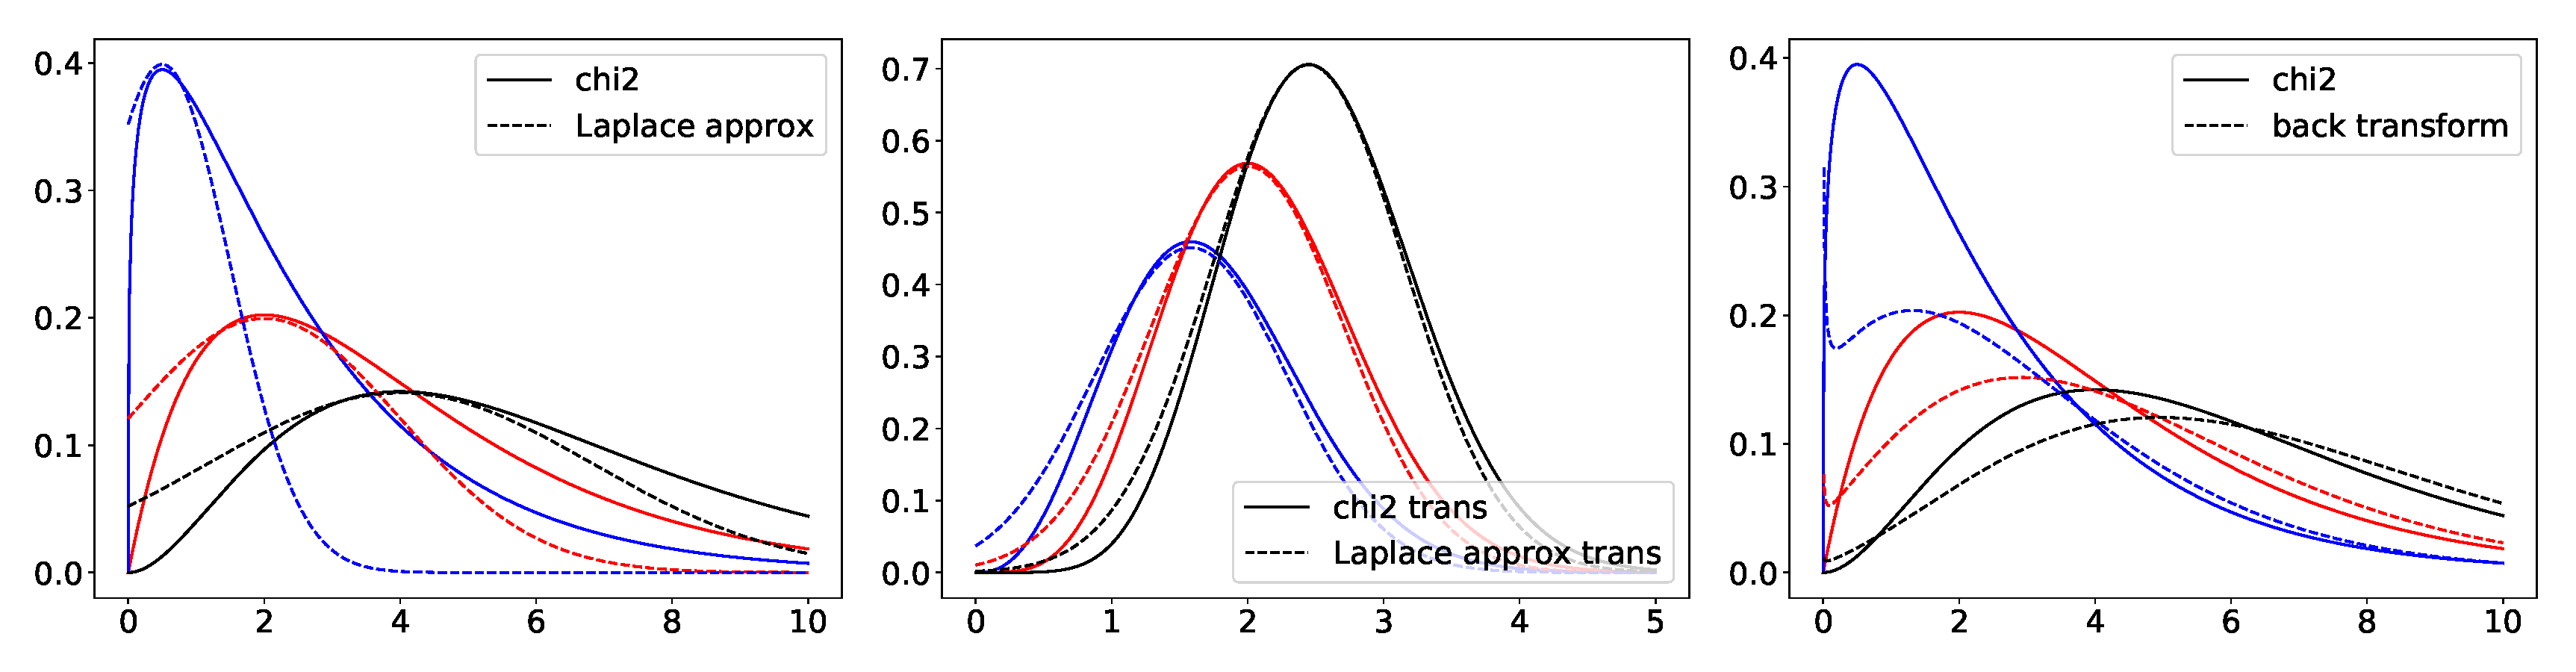
\includegraphics[width=\textwidth]{figures/chi2_playground_sqrt.pdf}
	\caption{chi2 sqrt comparison}
	\label{fig:chi2_sqrt_comparison}
\end{figure}